Factors that may limit estimation accuracy are discussed.
Clustering stability is analyzed as a potential contributor to the limited improvement from multiple features.

% \begin{figure}[t]
% 	\centerline{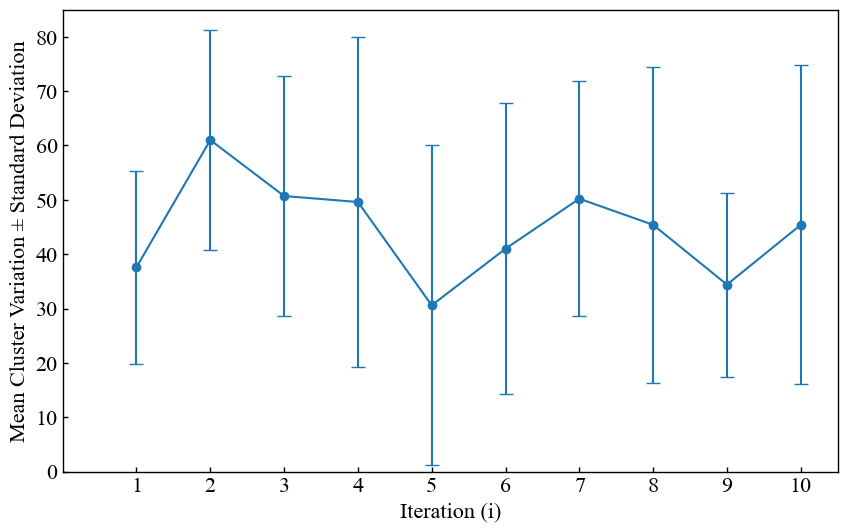
\includegraphics[width=\linewidth]{img/clustering.png}}
% 	\caption{Stability verification of cluster assignment for short video dataset}
% 	\label{fig:clustering-stability}
% \end{figure}

%
\revised{A random-inference baseline of 0.5 was used for binary classification.
Eight of the ten RF and XGBoost models exceeded the baseline on the short video dataset.
The result demonstrates that activity levels were estimated from point-cloud features.}

%
Section~\ref{subsec:evaluation-short} demonstrated that three-dimensional point-cloud features are effective for activity level estimation.
Clustering instability may partially explain the limited accuracy improvement from multiple features.
K-means clustering ($k$=3) was applied to the short video dataset as a baseline.
One sample was randomly removed and clustering was re-run 10 times per trial, repeated over 10 trials.
Cluster changes ranged from approximately 20 to 40 per trial.
Clustering instability is a contributing factor to the limited accuracy improvement from multiple features.
The XGBoost all-feature model achieved the highest accuracy in Section~\ref{subsec:evaluation-short}.
The accuracy gain over single-feature models remained limited.
A baseline clustering result was established with k-means ($k$=3) on the full dataset.
Mean and standard deviation of reassignment counts were computed across 10 trials of 10 removal-and-reclustering operations.
